
\documentclass{llncs}

\usepackage{graphicx}
\usepackage{url}

\usepackage{amsmath}

\begin{document}

%\conferenceinfo{WXYZ '05}{date, City.} 
%\copyrightyear{2011} 
%\copyrightdata{[to be supplied]} 

%\titlebanner{DRAFT---Do not distribute}        % These are ignored unless
%\preprintfooter{short description of paper}   % 'preprint' option specified.


\newcommand{\barc}{Barelogic$^S$}
\title{Performance of Parallel SAT Solvers}
\titlerunning{Parallel SAT}
\toctitle{Parallel SAT}
%\subtitle{Subtitle Text, if any, or comment out}

\author{Roberto As\'in Ach\'a\inst{1} \and Juan Olate \inst{2} \and Leo Ferres \inst{2}}

\institute{Departamento de Ingenier\'ia Civil Inform\'atica\\
  Facultad de Ingenier\'ia\\ Universidad Cat\'olica de la Sant\'isima
  Concepci\'on, Chile\\ \email{rasin@ucsc.cl} \and Department of
  Computer Science\\Faculty of Engineering\\Universidad de
  Concepci\'on, Chile\\ \email{\{lferres|juanolate\}@udec.cl}}


\maketitle

\begin{abstract}
This is the text of the abstract.
\end{abstract}

\section{Introduction}

In this paper, we study issues of scalability of parallel solvers of
the satisfiability (SAT) problem on hierarchical-memory multicore
(SMP) systems.

Since at least 2009, parallel SAT solvers (henceforth, pSATs) have
been performing at the top of the SAT Competition (in 2011, all three
wall-clock time winners of the competition are parallel solvers).
Also in 2011, pSATs and sequential SAT solvers are grouped into a
single competition
track\footnote{\url{http://www.satcompetition.org/}}, which signals
the widespread interest in pSATs by the research and industrial
communities. This appeal stems in part because of the inherent
properties of parallel algorithms, but also because of the need of 
the community to do better in other application domain and be able to 
handle even larger and more complex CNF formulas in smaller times 
taking advantage of modern hardware. 


Meanwhile, instead of increasing clock performance, chip manufacturers
are investing heavily on multicore architectures to improve
performance and lower power consumption (AMD released the 8-core
Opteron 3260 EE in late 2011, and Intel will do the same with the Xeon
E5-2650, and its low power version, the Xeon E5-2650L early this
year). As Herb Sutter once put it, ``the free lunch is over''
\cite{FreeLunchIsOver}, and it effectively means that software in
general will not be getting any faster as years go by simply
relying on faster processors, but by relying on how software scales in
over multicore systems.

Finally, modern memory architectures are not flat
Processor$\leftrightarrow$RAM architectures, but a hierarchy of
faster-but-smaller to slow-but-large memories with latencies varying
from 0.5{\it ns} access, 32{\it Kb} memories such as the L1 cache, to
tens of nanoseconds, megabyte-large memories like the L3 cache, to
gigabyte, 100{\it ns} access memory such as main memory. Hierarchical
memory architectures have a strong impact on the performance of
sequential software (e.g., row scanning arrays in row-major
representation, memory transfers may be in the order of the input
divided by the size of the cache line, while memory transfers for
column scanning is in the order of the square of the input). For
multicore systems, besides the problem of data representation, there
is the problem of false sharing: if two threads write on different
words of the same cache line, then the cache line in one or the other
processor becomes ``dirty'' and a round trip to RAM ensues, wasting
valuable time due to latency.

Thus, given the three arguments above: how {\em do} pSATs scale in
hierarchical-memory multicore architectures? Our case study is the
winner of the 2011 SAT Competition, {\tt plingeling}, a
portfolio-approach SAT solver \cite{lingeling}. The first experiment
tested a \emph{modified} \pling\ on a 6-core multicore machine,
varying the number of threads. \pling\ was modified in order that, for
each {\em thread worker}, the {\em same search} is performed
(i.e. same strategies, starting parameters and without lemma
exchanging).  In Figure \ref{fig:decay} we can see how
modified-\pling's performance tends to decay sharply (up to 30\%) when
several instances are executed in the same processor, even when they
do not, in principle, share any resources other than the common
process address space. We would thus expect that all instances would
perform similarly at 1, plus or minus a small fraction. This is in
fact what happens when \pling\ is run in two different cores of two
different chips, but in the same machine.

\begin{figure}[tp]
  \centering
  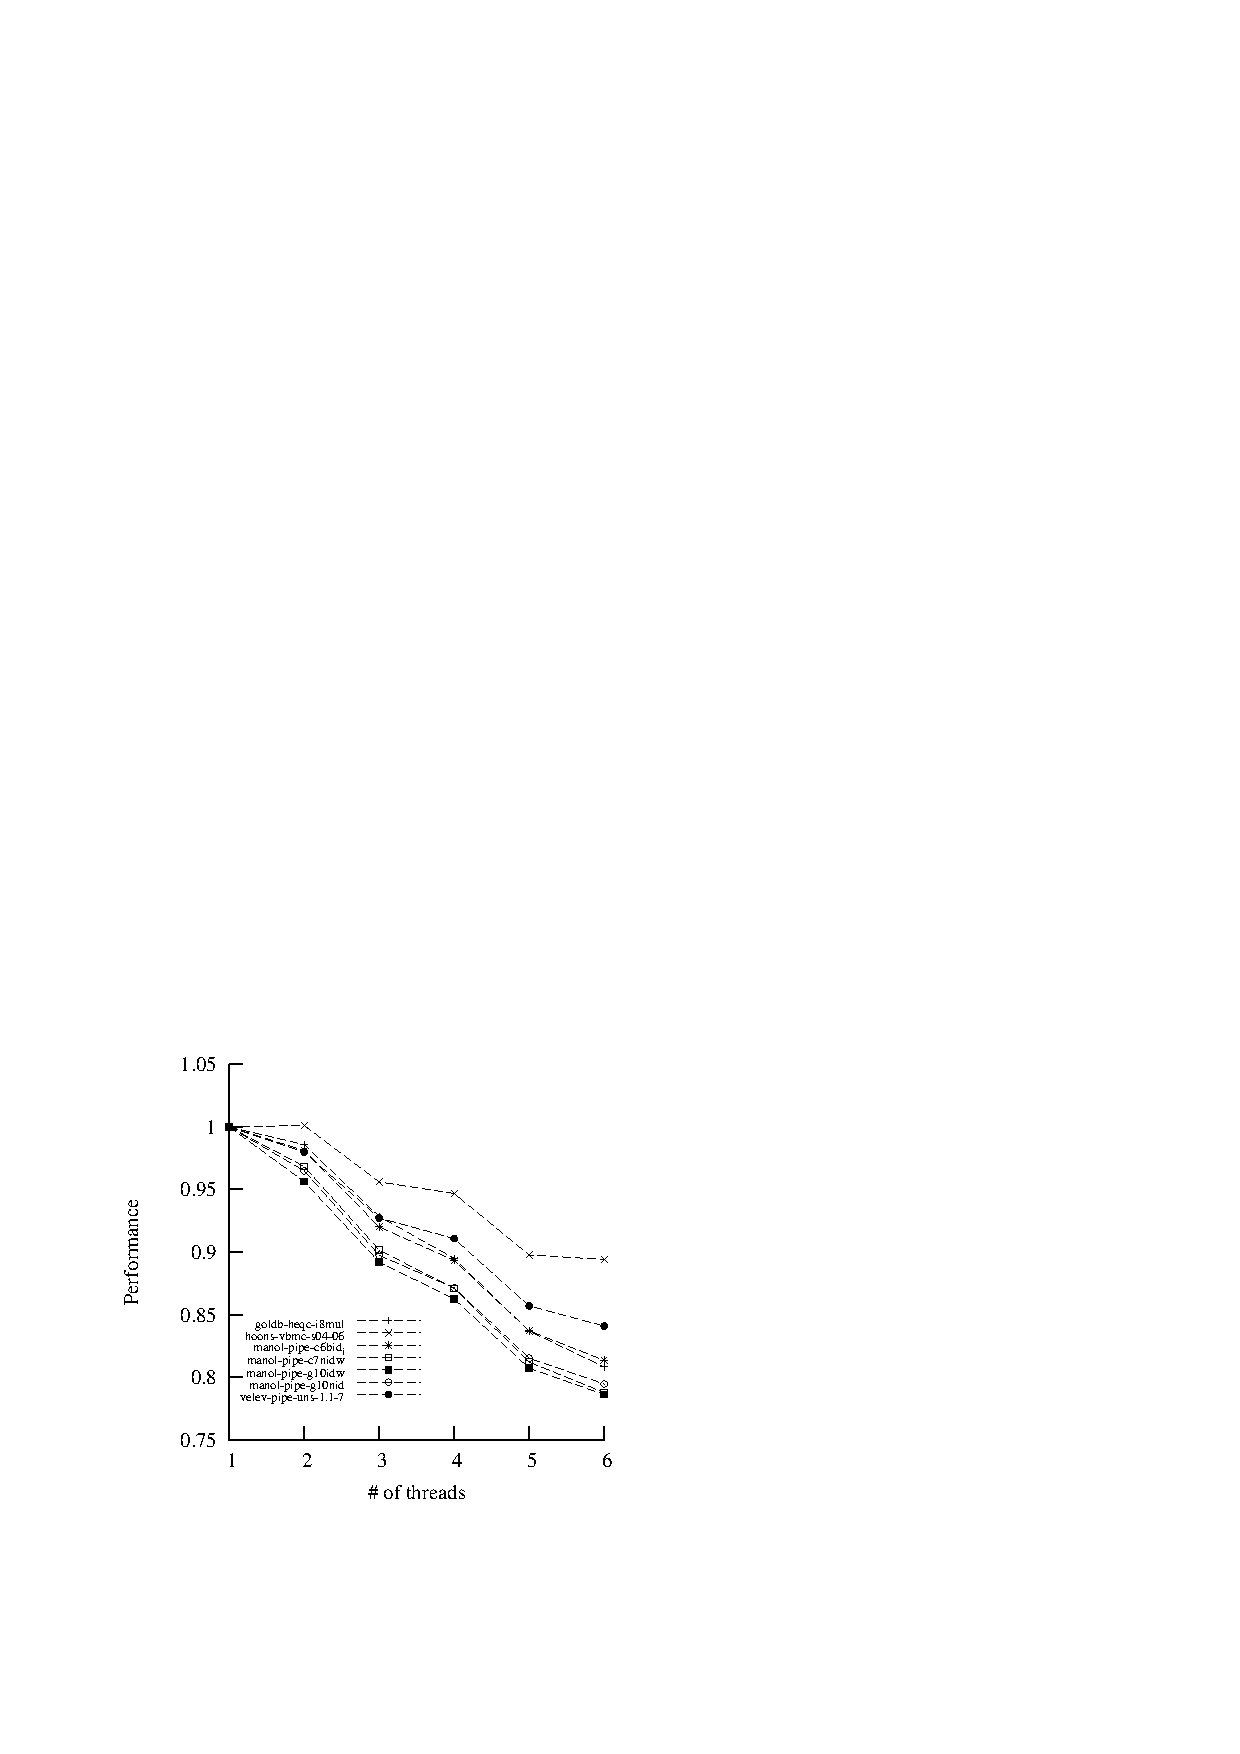
\includegraphics[scale=1]{plingeling_6cores_speedup}
  \caption{Performance decay of {\tt plingeling} when run over many cores}
  \label{fig:decay}
\end{figure}

In order to find the culprit of the performance decay, we have
developed a simple portfolio-based SAT solver that allows us to
replicate the behavior of \pling, and then also experiment with
alternative scenarios in order to take measures towards the
improvement of its performance.

In Section^\ref{} we.....

\section{Preliminaries}
\label{sec:preliminaries}
\subsection{SAT and SAT solvers}

A symbol $v \in V $ is known as a \emph{propositional variable} if $V$ is
 a fixed finite set of propositional symbols.  If $v \in V$,
then $v$ and $\lnot v$ are \emph{literals} of $V$.  
The \emph{negation} of a literal $l$, written $\lnot l$, denotes 
$\lnot v$ if $l$ is $v$, and $v$ if $l$ is $\lnot v$.
A \emph{clause} is a disjunction of literals $l_1 \lor\ldots\lor l_n$.
A \emph{unit clause} is a clause consisting of a single literal.  The
\emph{empty clause} is a clause that has no literals and will be
denoted by $\Box$.  A (CNF) \emph{formula} is a conjunction of one or
more clauses $C_1 \land\ldots\land C_n$. When it leads to no
ambiguities, we will sometimes also write such a formula in set
notation $\{C_1,\ldots,C_n\}$, or simply replace the $\land$
connectives by commas.  A (partial truth) \emph{assignment} $M$ is a
set of literals such that $\{ v, \lnot v \} \subseteq M$ for no $v$. A
literal $l$ is \emph{true} in $M$ if $l \in M$, is \emph{false} in $M$
if $\lnot l \in M$, and is \emph{undefined} in $M$ otherwise.  In this
paper $M$ will be written as a sequence (also seen as a set when
convenient) of literals with $M l$ meaning the concatenation of $M$
with $l$.   A clause $C$ is true in $M$ if at least one of its
literals is true in $M$.  It is false in $M$ if all its literals are
false in $M$, and it is undefined in $M$ otherwise. 
If $C$ is a clause $l_1
\lor\ldots\lor l_n$, we write $\lnot C$ to denote the formula $\lnot
l_1 \land\ldots\land \lnot l_n$.
Hence, the empty
clause is always false.  A formula $F$ is true in $M$, or
\emph{satisfied} by $M$, denoted $M\models F$, if all its clauses are
true in $M$.  In that case, $M$ is a \emph{model} of $F$.  If $F$ has
no models then it is \emph{unsatisfiable}.  

The problem we are interested in is the \emph{SAT problem}: given a
formula $F$, decide whether there exists a model that satisfies
$F$.
Since there exists a polynomial transformation
(see~\cite{Tseitin1968}) for any arbitrary formula to an
equisatisfiable CNF one, we will assume w.l.o.g. that $F$ is in CNF.

A software program that solves this problems is called a \emph{SAT solver}
The Conflict-Driven-Clause-Learning (CDCL) algorithm, is nowadays at the 
basis of most state-of-ther-art SAT-solvers\cite{EenSorensson2003SAT,
picosat2008,rsat,siege, plingeling}. This algorithm has, at its roots, the very 
simple DPLL algorithm~\cite{Davisetal1962CACM}. Thanks to the work done, mainly,
 in \cite{relsat,Chaff2001, GRASP1999IEEE, ZhangStickel1996IMATH} it has evolved
 to an algorithm that incorpores several conceptual and implementation 
improvements, making modern SAT-solvers able to handle formulas of millons 
of variables and clauses. In \ref{} we sketch the CDCL algorithm.


\IncMargin{1em}
\begin{algorithm}
  \SetKwData{Cost}{cost}\SetKwData{J}{j}\SetKwData{Core}{core}
  \SetKwData{Result}{res}\SetKwData{BV}{BV}
  \SetKwInOut{Input}{Input}\SetKwInOut{Output}{Output}
  \Input{formula $F=\{C_1,\ldots,C_m\}$}
  \Output{SAT OR UNSAT}
  \BlankLine
  \Cost \assign 0\;
  \J \assign 1\;
  $F_w$ \assign $F$\;
  \While{true}{
    \While{ \Conflict \assign PROPAGATE() }( 
      \lIf{ DECISION\_LEVEL == 0 }( \Return UNSAT\;)
      \Lemma \assign CONFLICT\_ANALYSIS(\Conflict)\;
      \Lemma \assing LEMMA\_SHORTENING(\Lemma)\;
      LEMMA\_LEARNING(\Lemma)\;
      \Dl \assign LARGEST\_DL(\Lemma)\;
      BACKJUMP(\Dl)\;
    }
    
  \Dec \assign DECIDE()\;
    \lIf{ \Dec = 0 }(\Return SAT\;)
    DECIDE( \Dec )\;
  }
  \caption{CDCL algorithm}\label{alg:CDCL}
\end{algorithm}\DecMargin{1em}

As can be seen ..... explain and link concepts of the algorithm.

For a complete review of this algorithm as well as proofs over its termination and soundness we refer to \cite{Niewuenhuiss. }


\subsection{Parallel SAT solvers}

\section{Cache performance in Plingeling}
\section{Azudici}
\label{sec:azudici}

\section{Cache Performance in Azudici}

\section{Related Work}

\section{Conclusions and Future Work}
\appendix
\section{Appendix Title}

This is the text of the appendix, if you need one.

Acknowledgments, if needed.

% We recommend abbrvnat bibliography style.
\bibliographystyle{abbrvnat}

% The bibliography should be embedded for final submission.
\bibliography{bitap}

\end{document}
